\documentclass{report}
\usepackage{setspace}
\usepackage{graphicx} % Required for inserting images
\usepackage{caption}
\usepackage{subcaption}
\usepackage{amsmath} 
\usepackage[toc,page]{appendix}
\usepackage{adjustbox}
\usepackage{listings}
\usepackage{pgfplots}
\usepackage{makecell}
\usepackage{csvsimple}
\usepackage{physics}
\usepackage{cleveref}
\usepackage[dvipsnames]{xcolor}
%\definecolor{deepgray}{rgb}{.3,.3,.3}
\definecolor{deepblue}{rgb}{0,0,0.5}
\definecolor{deepred}{rgb}{0.6,0,0}
\definecolor{deepgreen}{rgb}{0,0.5,0}
\definecolor{foamC}{rgb}{0,1,1}
\lstset{frame=tb,
        numbers=left,
        basicstyle=\footnotesize\ttfamily,
        keywordstyle=\color{deepblue}\bfseries\ttfamily,
        stringstyle=\color{deepred}\ttfamily,
        commentstyle=\color{deepgreen},%\itshape\ttfamily,
        morecomment=[l][\color{magenta}]{\#},
        showstringspaces=false,
        breaklines=true,
        emphstyle=\bfseries\ttfamily}

\graphicspath{{Figures/}}

\usepackage[		% use biblatex for bibliography
backend=biber,      % use biber or bibtex backend
style=authoryear,   % choose style
natbib=true,		% allow natbib commands
hyperref=true,	    % activate hyperref support
alldates=year,      % only show year (not month)
]{biblatex}

\addbibresource{hw2writeup.bib}


\renewcommand{\chaptername}{Problem}

\title{Homework 2}
\author{Abbie Brunner}
%\date{February 22, 2024}

\onehalfspacing
\begin{document}

\maketitle

\tableofcontents

\chapter{}

\section{Part A}

The first part of this problem involves finding the complex potential function for a flow with stagnation points at $(1, 0), (0, 1), (-1, 0),\text{ and }(0, -1)$
If we take the basic form of the source/sink complex potential function

\begin{equation}
   F(z) = \frac{Q}{2\pi}\ln(z-z_0)
   \label{sink}
\end{equation}

where we cycle $z_0$ through each stagnation point in the form $z_0 = x_0 + iy_0$we can simply use a superposition of potential flows:

\begin{equation}
   F(z) = \frac{Q}{2\pi}\sum_{n = 1}^{4} \ln(z-z_n)
   \label{complexp1}
\end{equation}

\section{Part B}

To find the expressions for $\psi(x, y) \text{ and } \phi(x, y)$ we return to the basic form of the source/sink potential function

\begin{equation}
   F(z) = \frac{Q}{2\pi}\ln(z), \qquad z = re^{\theta i}
   \label{basic}
\end{equation}

By plugging in this definition of $z$ we find that

\begin{equation}
   F(z) = \frac{Q}{2\pi}\ln(r)+\frac{Q\theta}{2\pi}i, \qquad F = \phi + i\psi
   \label{polarcomp}
\end{equation}

Taking the imaginary part of this function gives us $\psi$, the function of the streamlines, and we can convert to cartesian using $\theta = \atan(\frac{y}{x})$
Similarly, the real part of the function gives us $\phi$, the velocity potential, and can be converted with $r^2 = x^2+y^2$

\begin{equation}
   \psi(x, y) = \frac{Q}{2\pi}\atan(\frac{y}{x}), \qquad \phi(x, y) = \frac{Q}{4\pi}\ln(x^2+y^2)
   \label{cartfunc}
\end{equation}

Finally, these functions can be transposed in a similar way to the original complex function by using $y-y_0 \text{ and } x-x_0$

\clearpage

\section{Part C}

\begin{figure}[!h]
   \centering
   \begin{subfigure}{0.5\textwidth}
      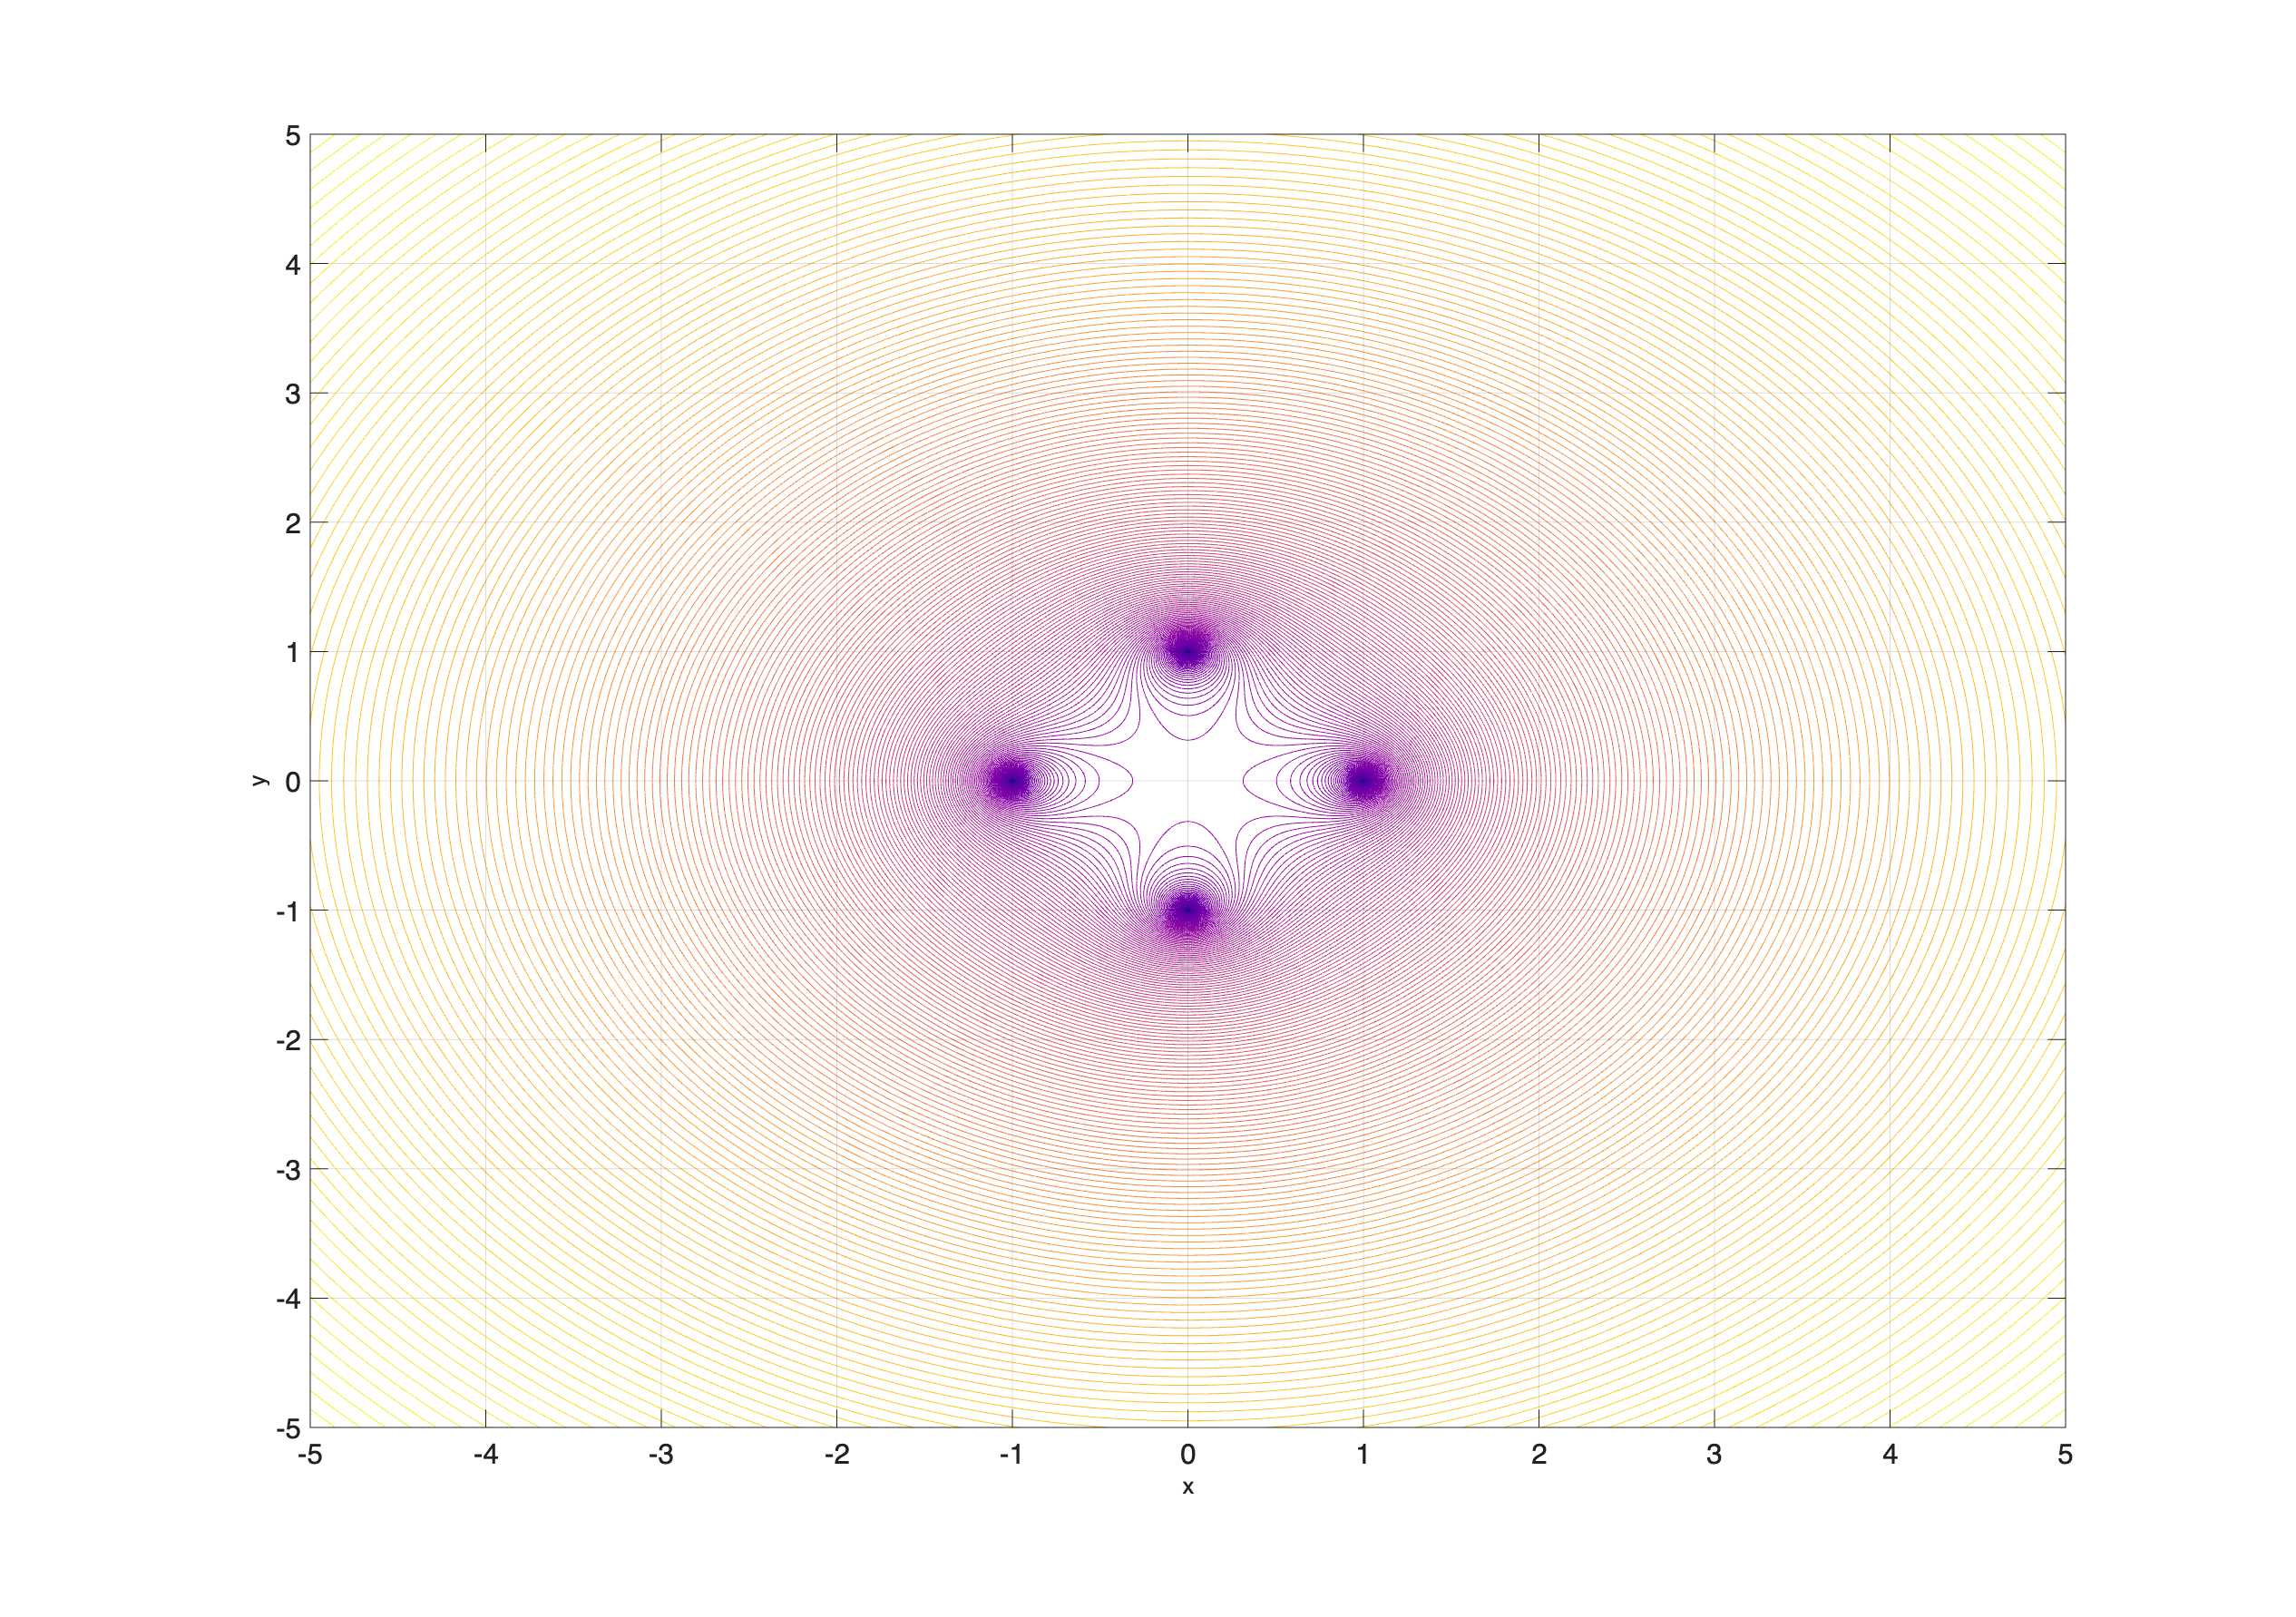
\includegraphics[width=\textwidth]{p1pot.eps}
      \caption{Velocity Potential Function}
      \label{velpotplot}
   \end{subfigure}
   \begin{subfigure}{0.5\textwidth}
      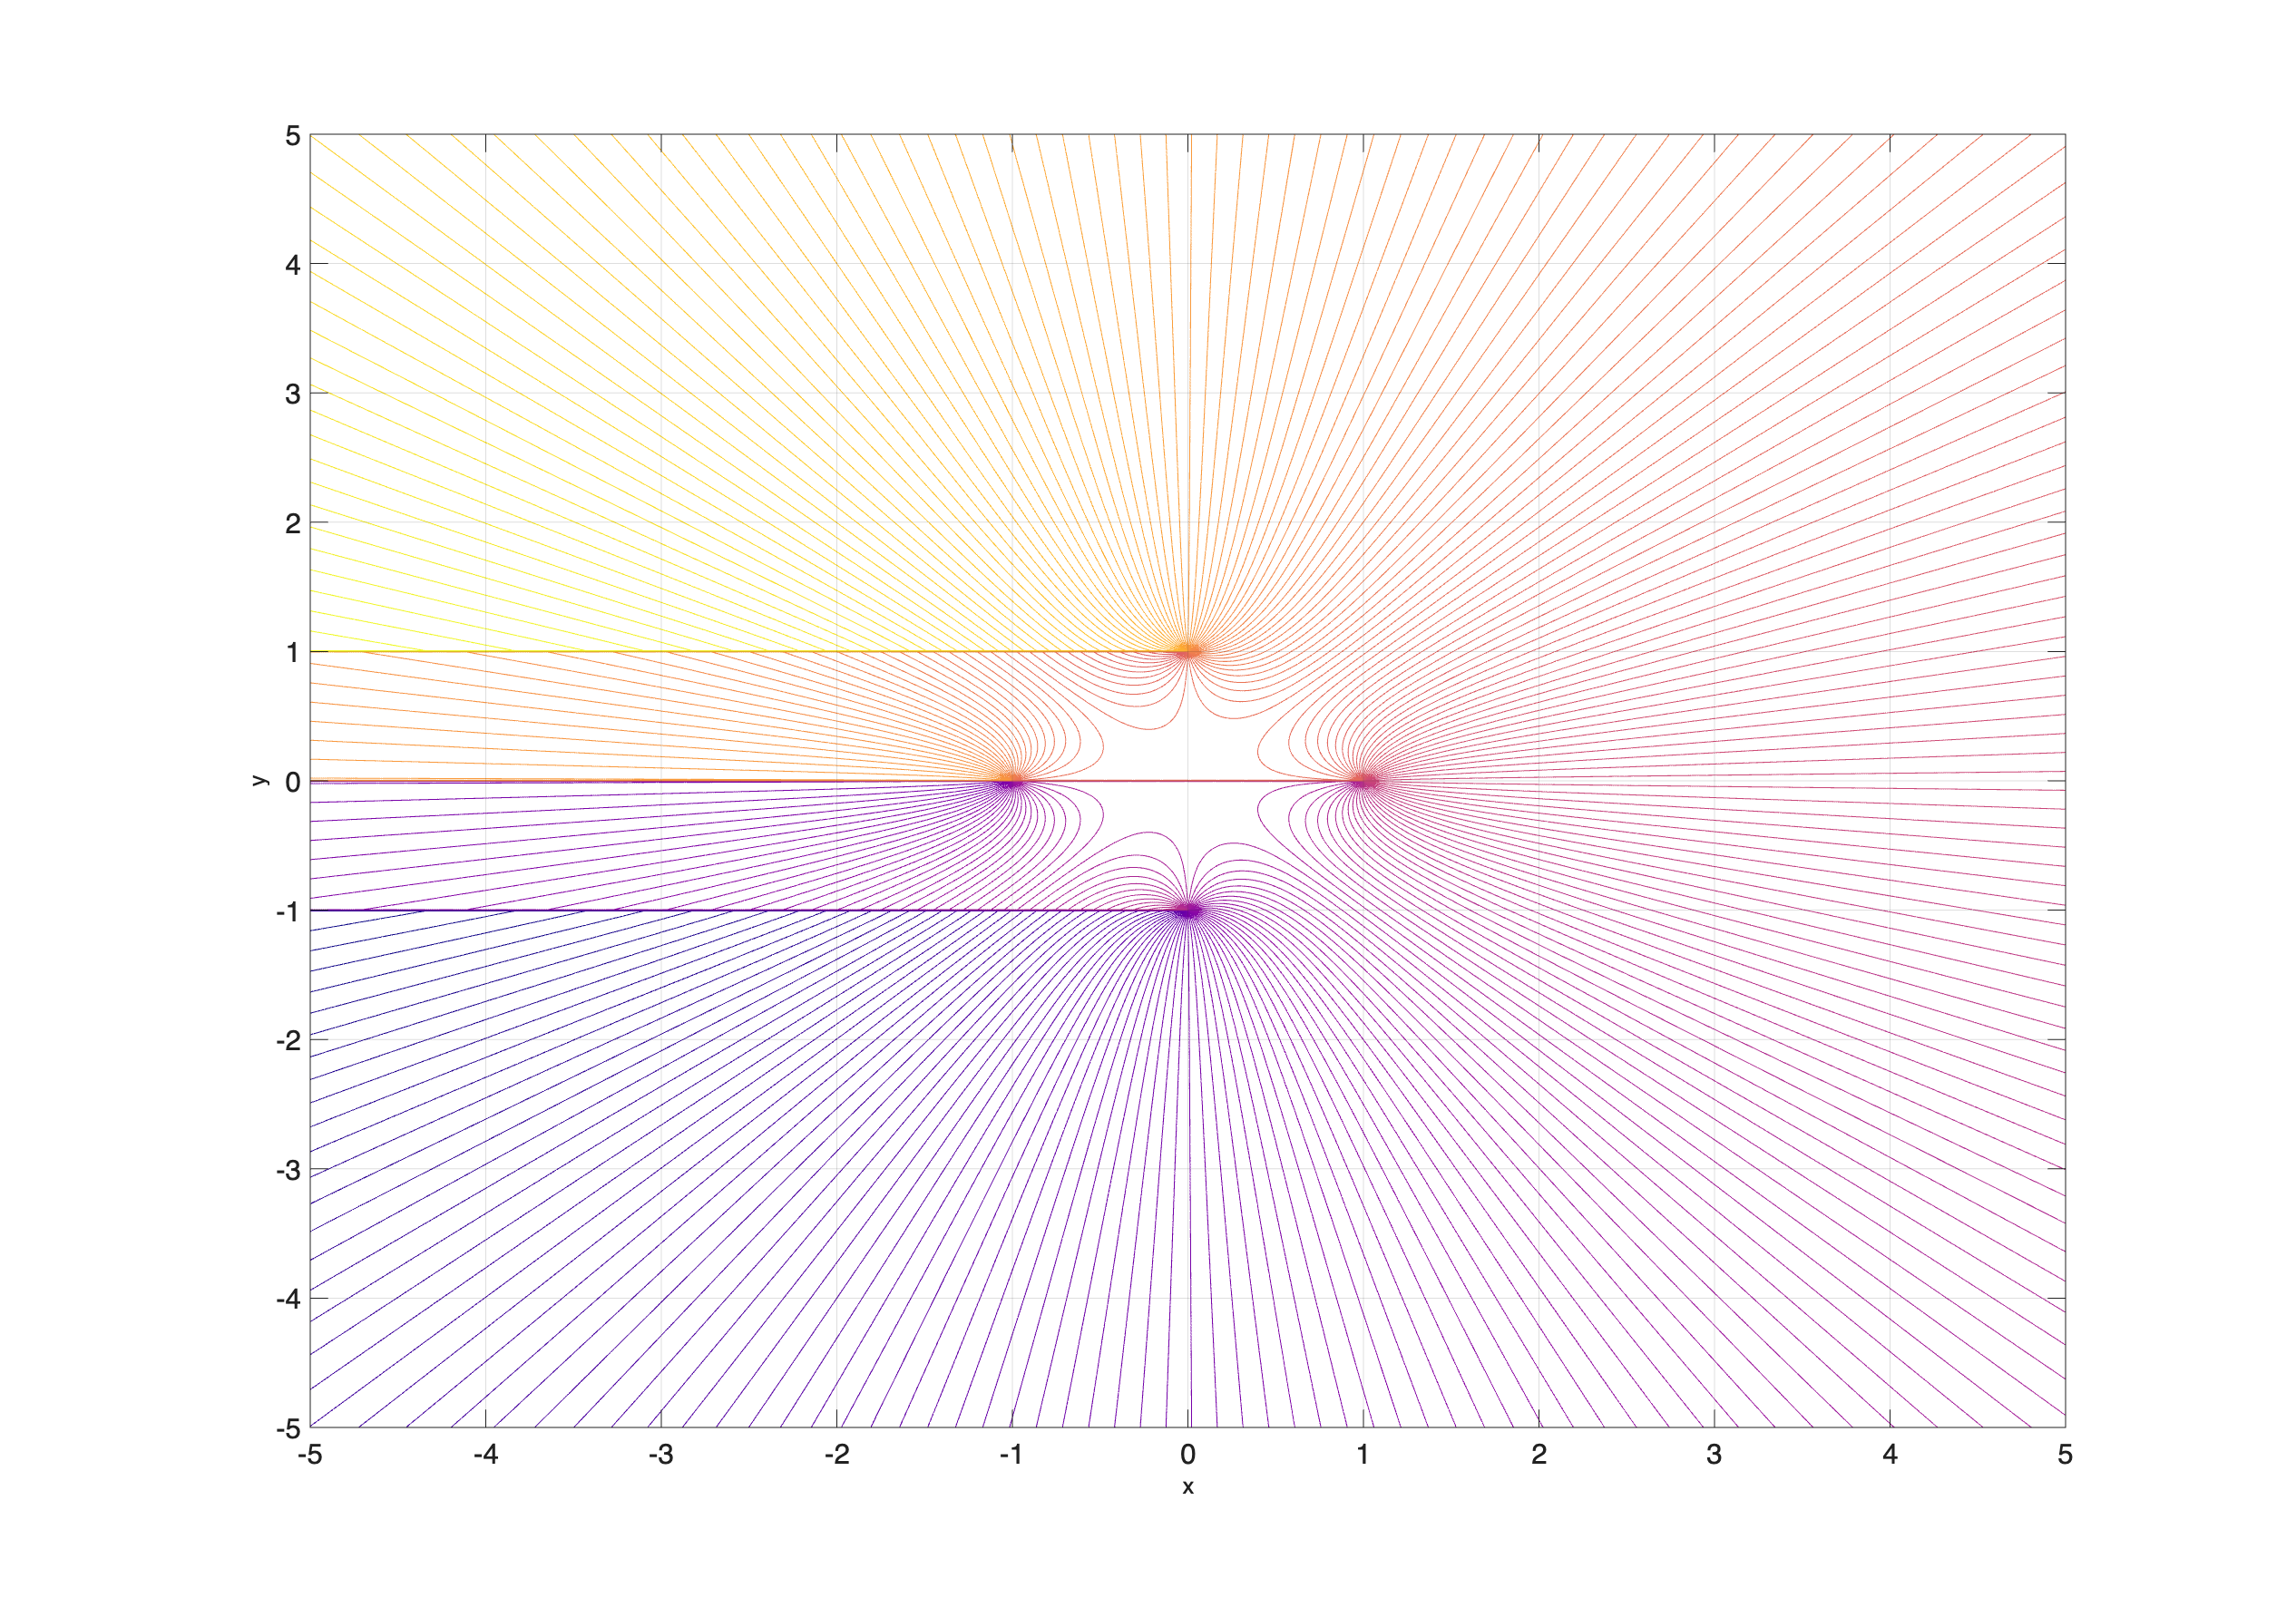
\includegraphics[width=\textwidth]{p1stream.eps}
      \caption{Streamline Function}
      \label{streamplot}
   \end{subfigure}
   \caption{Streamlines and Velocity Potential}
   \label{p1partc}
\end{figure}

\section{Part D}

Using the provided streamfunction find the velocity components at $(0, 1) \text{ and } (2, 4)$

\chapter{}

\section{Part A}

An initial read of this problem indicates that general superposition can be used with a corner flow and a vortex

\begin{equation}
   F(z) = Uz^{\frac{5}{3}} - \frac{i\Gamma}{2\pi}\ln(z-z_0), \qquad \text{where} \quad z_0 = a\cos(\alpha)+i\sin{\alpha}
   \label{comppotbad}
\end{equation}

However plotting this result presents a problem. Looking at \cref{potbad} we see that the streamlines cross the x-axis.

\begin{figure}
   \centering
   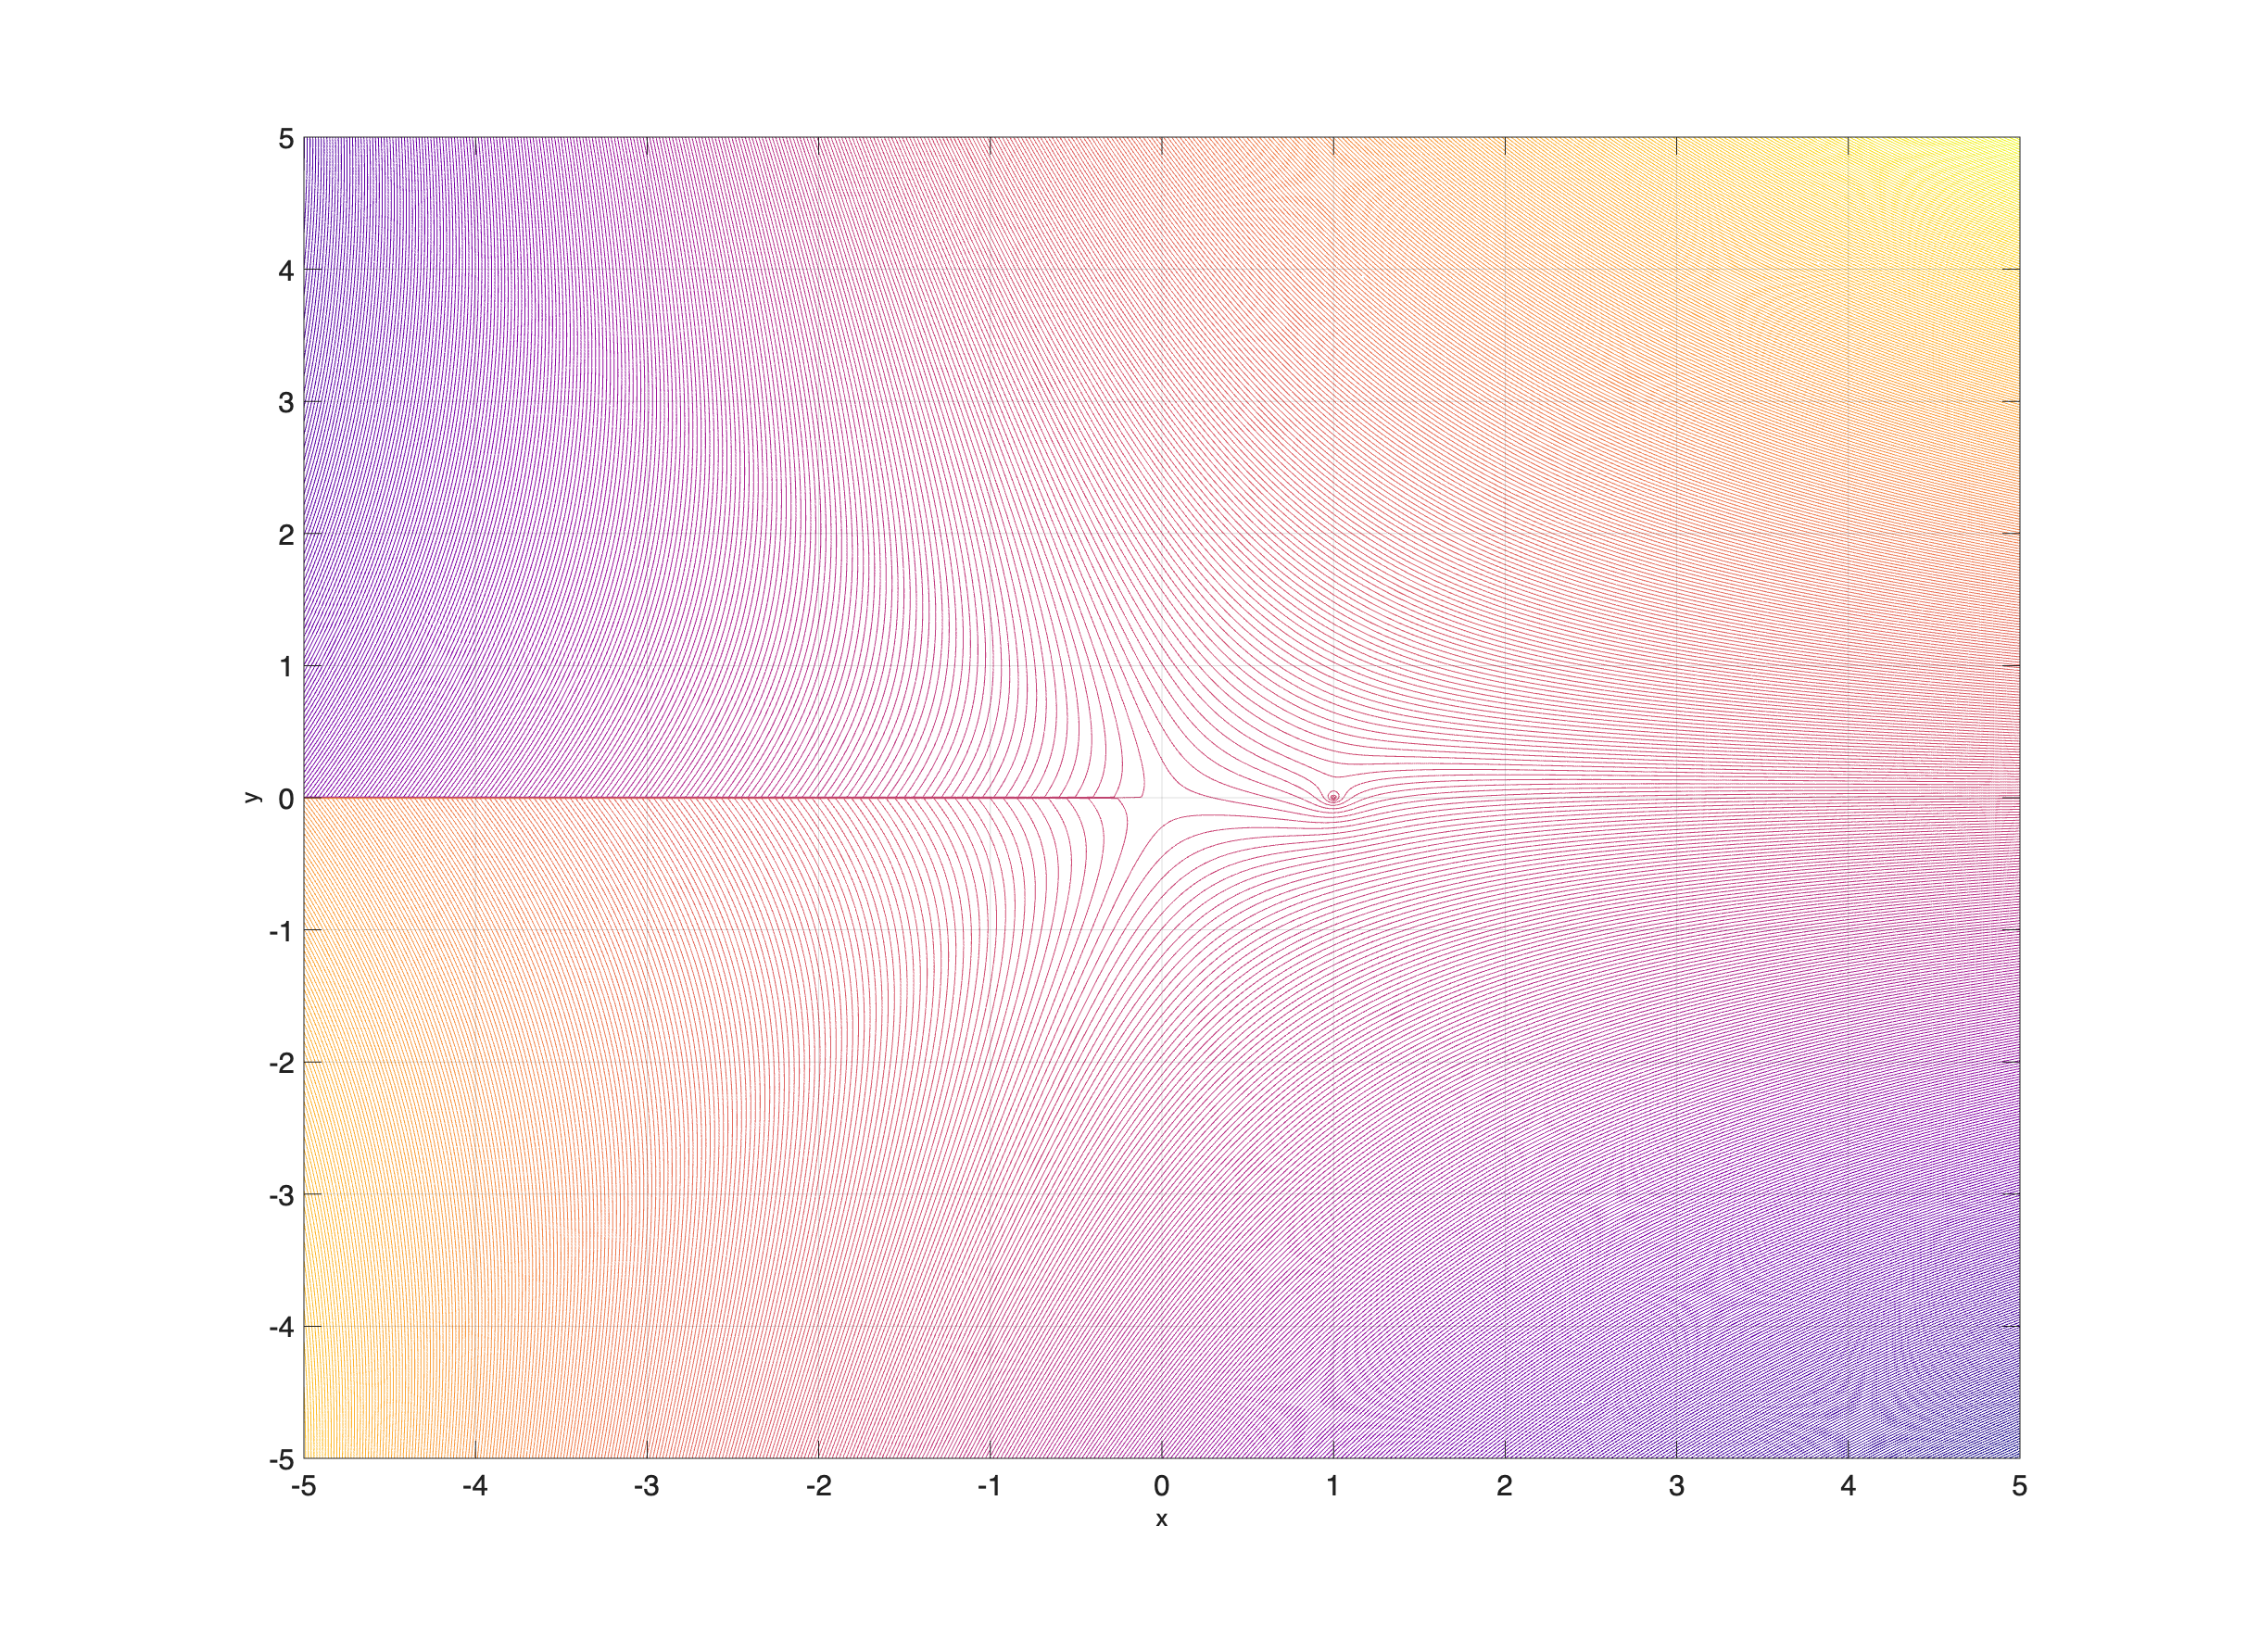
\includegraphics[width=0.85\textwidth]{p2streambad.eps}
   \caption{Superimposed Streamlines}
   \label{compbad}
\end{figure}

To fix this we can try using a map from a $\zeta$ plane to a $z$ plane.
The $\zeta$ map will be two counter-rotating vortices in a uniform flow.

\begin{equation}
   F(\zeta) = U\zeta - \frac{i\Gamma}{2\pi}\qty(\ln(z+z_0)+\ln(z-z_0))
   \label{zetaflow}
\end{equation}

To kick the x axis to the angle that we desire in the corner we can use the map of

\begin{equation}
   \zeta = G(z) = z^\frac{3}{2}
\end{equation}

This yields the result that we are after as seen in \cref{problem2}

\section{Part C}

\begin{figure}[!h]
   \centering
   \begin{subfigure}{0.65\textwidth}
      \centering
      
\includegraphics[width=\textwidth]{p2pot.eps}
      \caption{Velocity Potential}
      \label{p2pot}
   \end{subfigure}
   \begin{subfigure}{0.65\textwidth}
      \centering
      
\includegraphics[width=\textwidth]{p2stream.eps}
      \caption{Streamfunction}
      \label{p2stream}
   \end{subfigure}
   \caption{Problem 2 Plots}\
   \label{problem2}
\end{figure}

\chapter{}

\section{Part A}

For this setup we can use the superposition of three flows.
Using the flow of a doublet, uniform flow, and a source at the location specified.

\begin{equation}
   F(z) = \frac{\mu}{z}+Uz+\frac{Q}{2\pi}\ln(z-z_0), \qquad z_0 = 2a+0i
   \label{part3comp}
\end{equation}

\section{Part B}

We can compute the forces on the cylinder by using Blasius' Theorem.

\begin{equation}
   f_x-if_y=i\frac{\rho}{2}\oint W^2 \,dz
   \label{bt}
\end{equation}

\section{Part C}

\begin{figure}[!h]
   \centering
   \begin{subfigure}{0.65\textwidth}
      \centering
      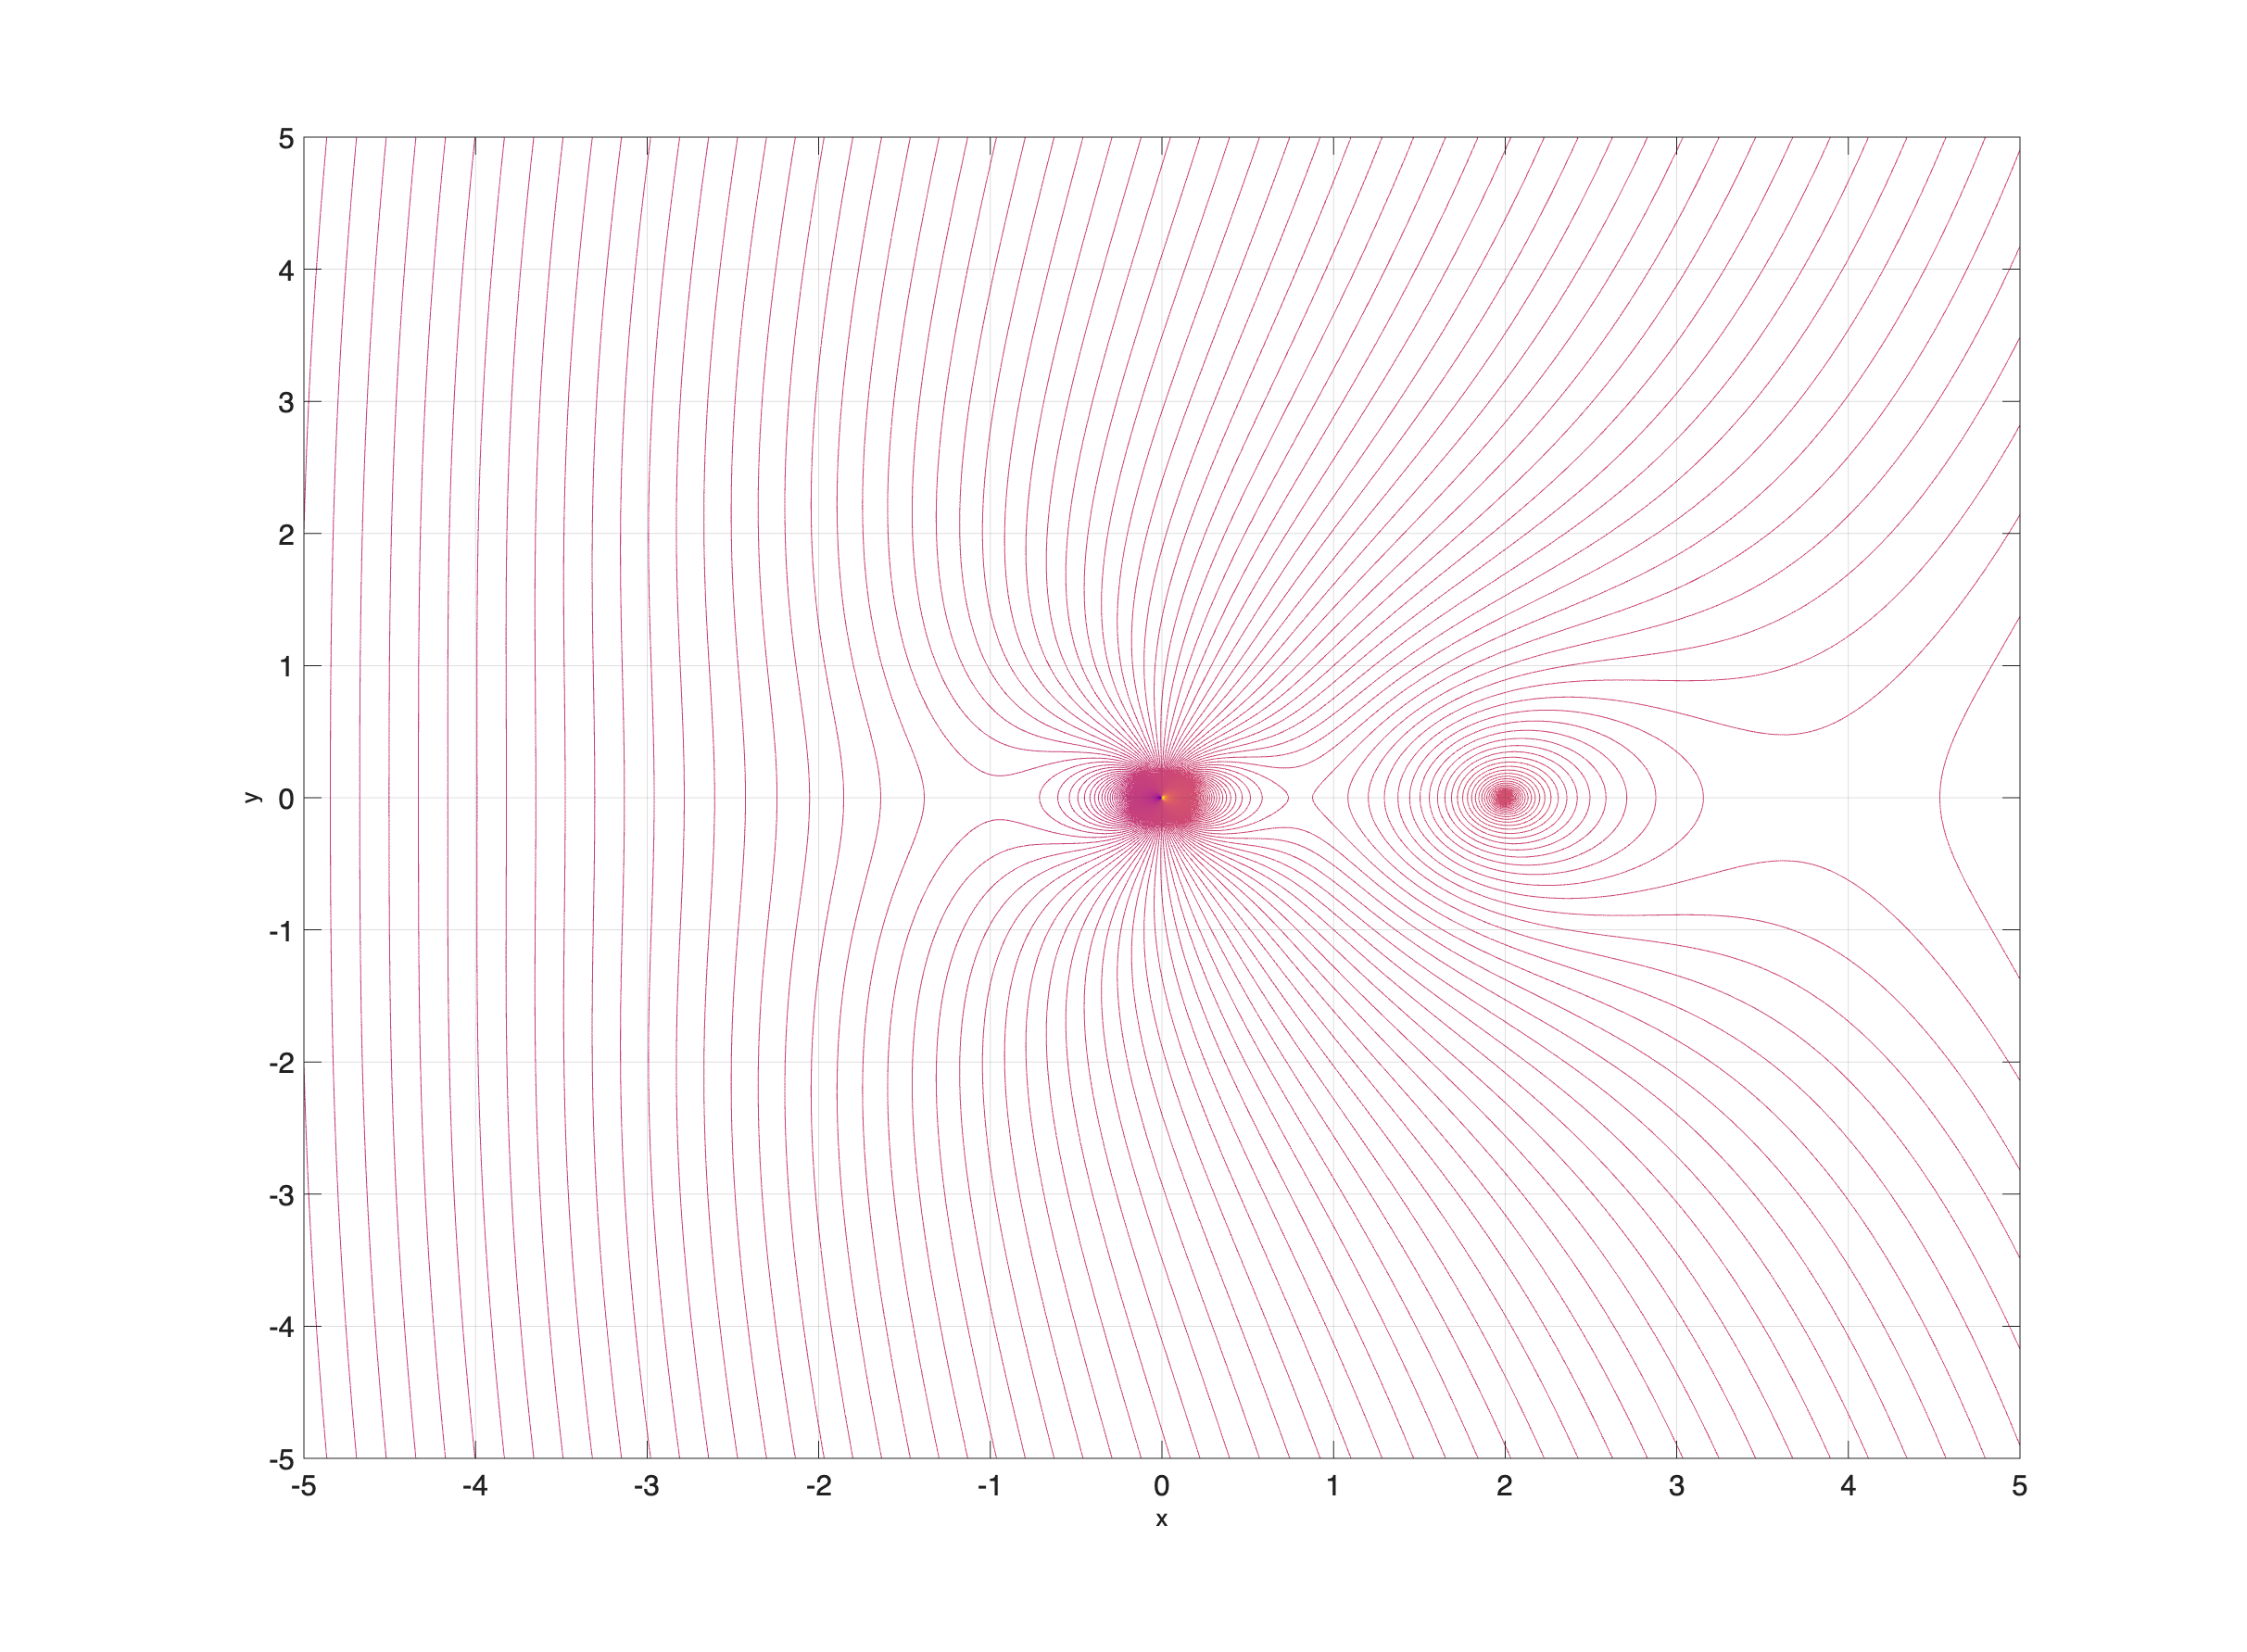
\includegraphics[width=\textwidth]{p3pot.eps}
      \caption{Velocity Potential}
      \label{p3pot}
   \end{subfigure}
   \begin{subfigure}{0.65\textwidth}
      \centering
      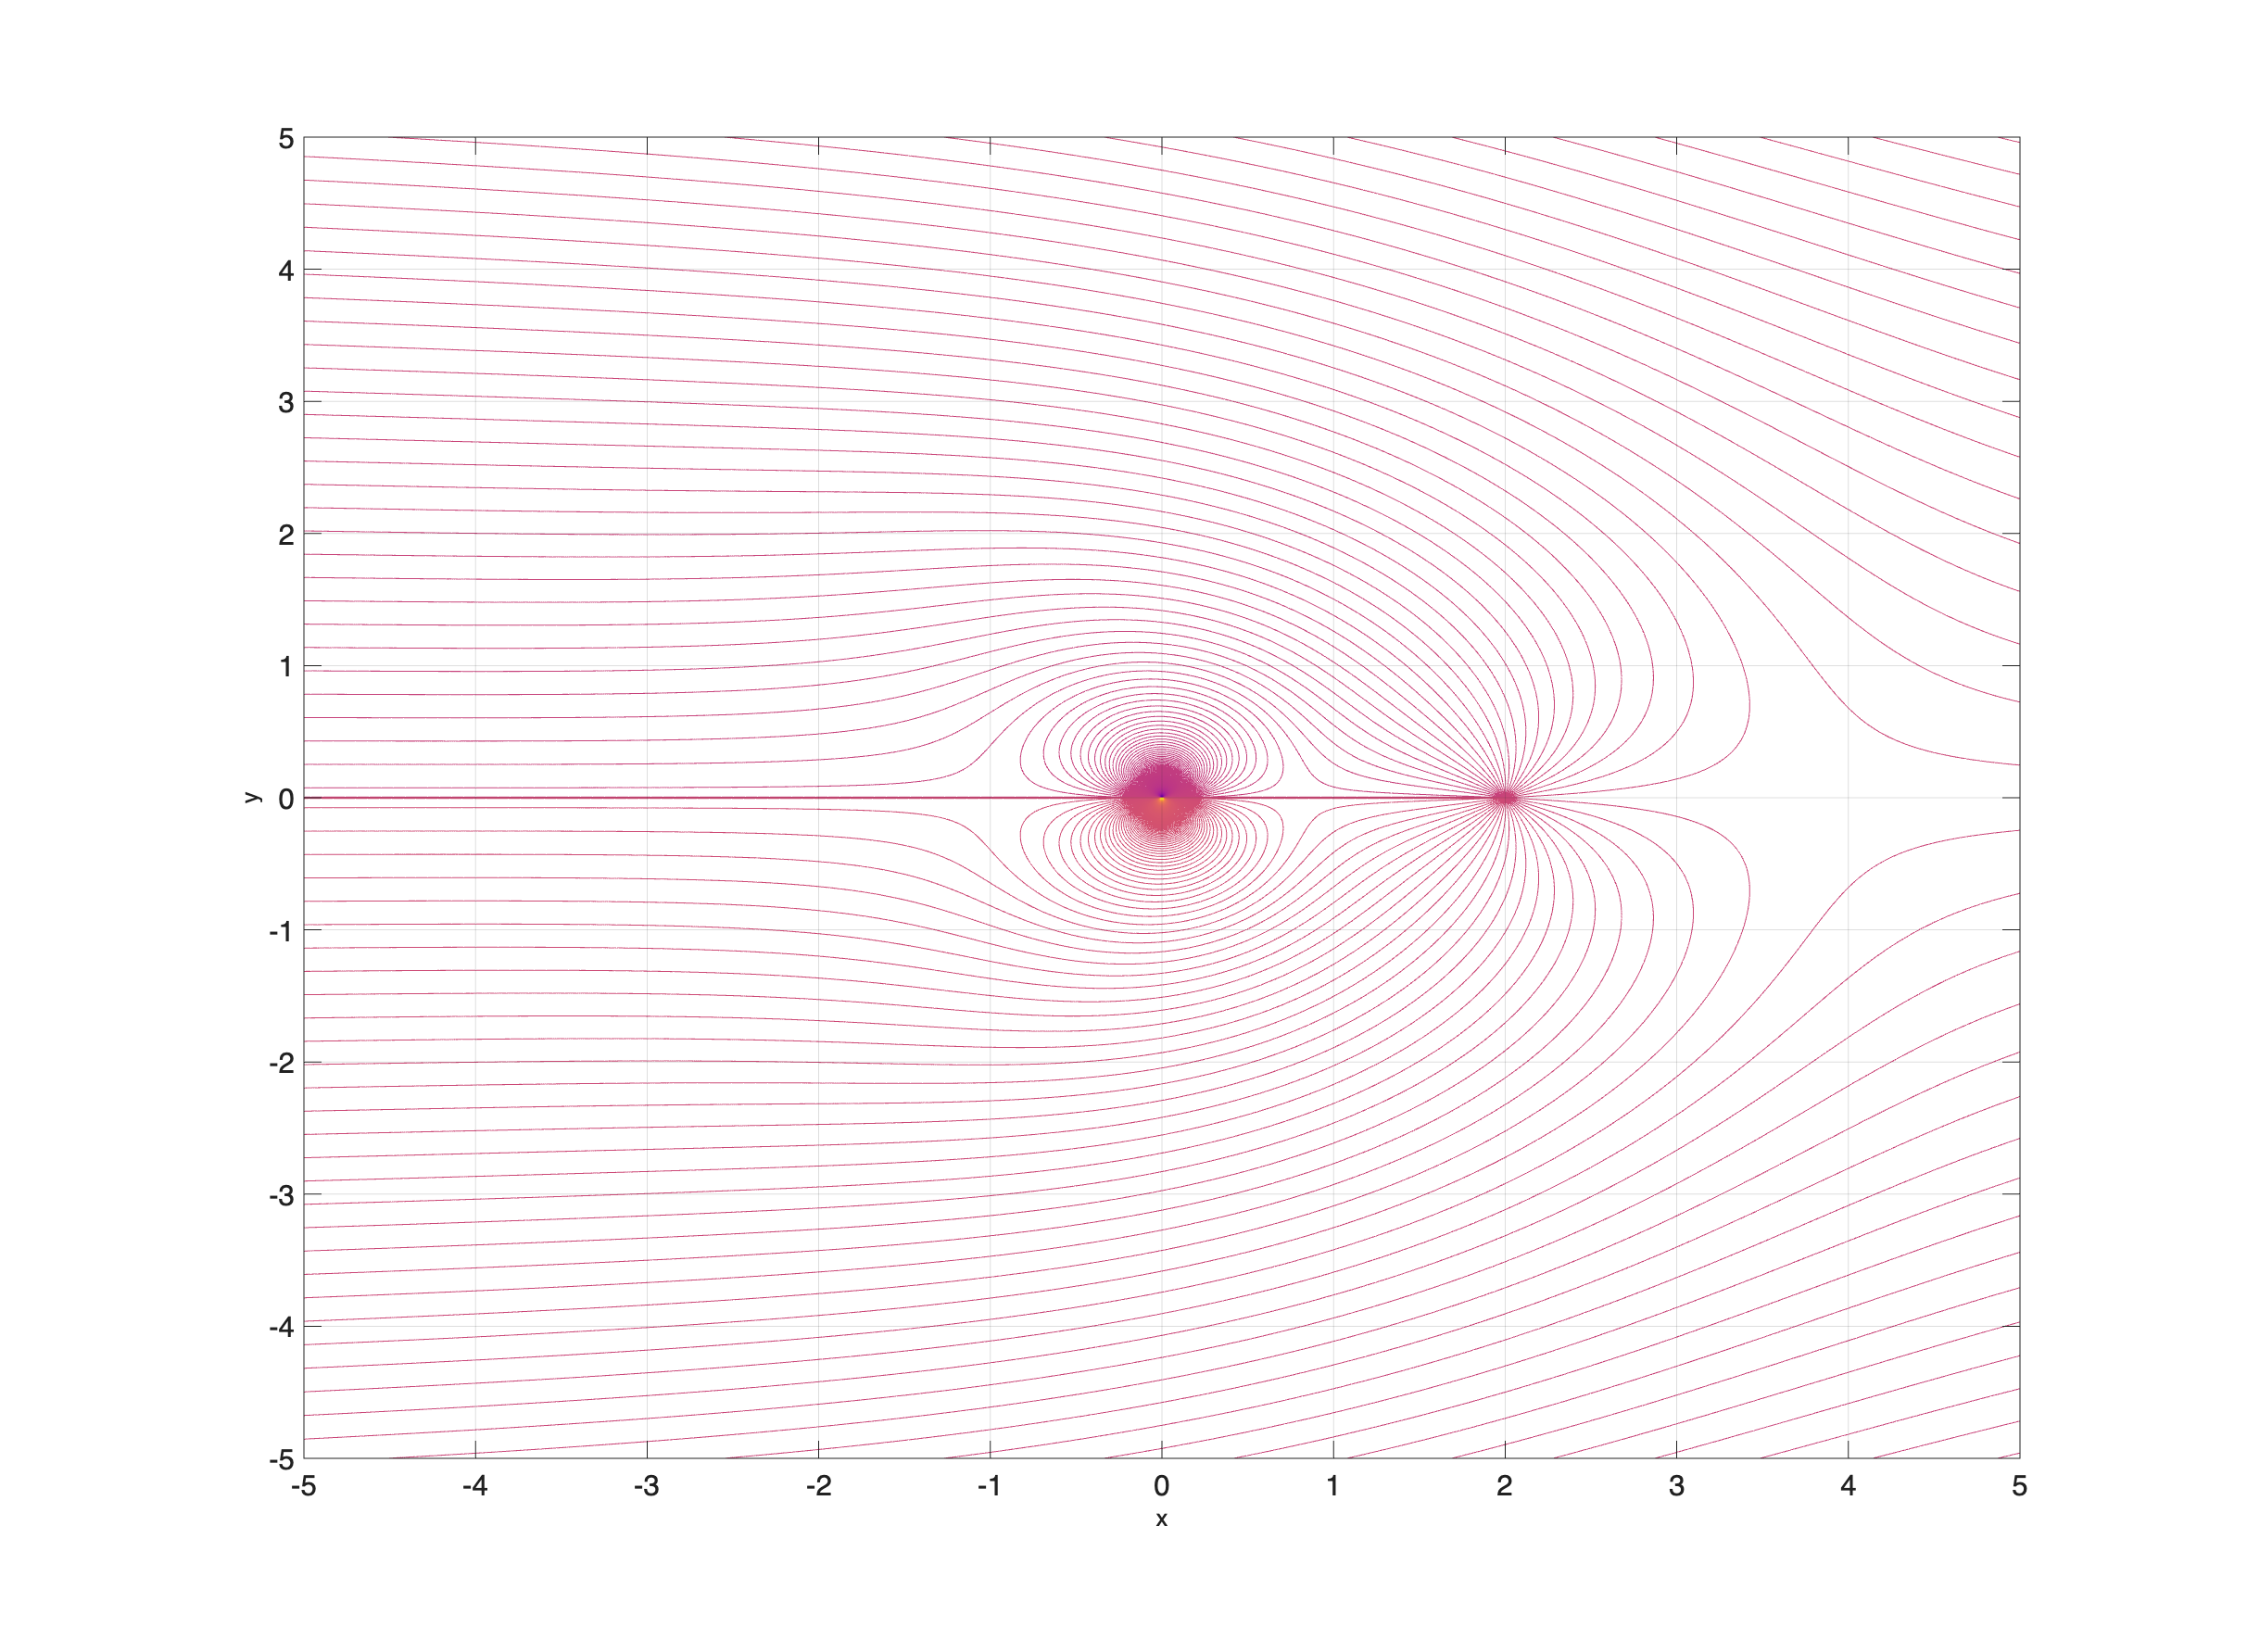
\includegraphics[width=\textwidth]{p3stream.eps}
      \caption{Streamfunction}
      \label{p3stream}
   \end{subfigure}
   \caption{Problem 3 Plots}\
   \label{problem2}
\end{figure}



\clearpage

\appendix

\chapter{Problem 1 Code}
   \lstinputlisting[language=Matlab,numbers=none]{HW2P1.m}
\chapter{Problem 2 code}
   \lstinputlisting[language=Matlab,numbers=none]{HW2P2.m}
\chapter{Problem 3 code}
   \lstinputlisting[language=Matlab,numbers=none]{HW2P3.m}

\end{document}
